\documentclass[tikz]{standalone}

% \usepackage{newtxtext,newtxmath}

% mytikzset
\usepackage{tikz}
\usetikzlibrary{positioning,arrows,shapes}
\usetikzlibrary{decorations.pathmorphing}
\usetikzlibrary{decorations.markings}
\usetikzlibrary{shapes.arrows, fadings}
\usetikzlibrary{shapes,snakes}
\usetikzlibrary{calc}

\tikzset{
  vector/.style={thick,double,draw=black, postaction={decorate},
    decoration={markings,mark=at position .6 with {\arrow[black,scale=0.4]{triangle 45}}}},
  axial/.style={thick,double,densely dashed,draw=black, postaction={decorate},
    decoration={markings,mark=at position .6 with {\arrow[black,scale=0.4]{triangle 45}}}},
  gluon/.style={decorate, draw=black,
    decoration={coil,aspect=0.3,segment length=5pt,amplitude=3pt}},
  pseudo/.style={thick, dashed, draw=black, postaction={decorate},
    decoration={markings,mark=at position .6 with {\arrow[red,scale=0.5]{triangle 45}}}},
  scalar/.style={thick,draw=black, postaction={decorate},
    decoration={markings,mark=at position .6 with {\arrow[black,scale=0.5]{triangle 45}}}}%,
  % pomeron/.style={thick,draw=black, postaction={decorate},
  % decoration={zigzag,segment length=4,amplitude=.9}}
}


\definecolor{cola}{rgb}{0.9,0.62,0.0}
\definecolor{colb}{rgb}{0.337, 0.706, 0.914 }
\definecolor{colc}{rgb}{0.0, 0.62, 0.451}

\begin{document}
\nopagecolor
  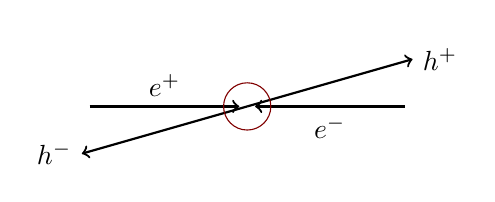
\begin{tikzpicture}[node distance=0.7cm and 1.0cm, baseline=1cm]
%
    % \foreach \a in {-10,-8.7,...,10} :
    %   \draw[very thin, black!20!white] (0, 0) -- ({10/\a}:1.3)  ;
    % \foreach \a in {-10,-8.77,...,10} :
    %   \draw[very thin, black!20!white] (0, 0) -- ({180+10/\a}:1.3);
%
    \draw[->,thick] (-2, 0) -- node[above] {$e^+$} (-0.1, 0);
    \draw[->,thick] ( 2, 0) -- node[below] {$e^-$} (0.1 ,0);
%
    % \node[coordinate] (vLb) at (0.5 ,0.5) {};
    \draw[->,thick] ( 0.0, 0.0) -- (2.1, 0.6) node[right] {$h^{+}$};
    \draw[->,thick] (-0.0,-0.0) -- (-2.1, -0.6) node[left] {$h^{-}$};
    % \draw[] (vLb) -- (3.5, 0.7) node[right] {$p$};
    % \draw[] (vLb) -- (3.7, 0.6) node[right] {$K^-$};
    % \draw[] (vLb) -- (4.8, 0.2) node[right] {$\mu^+$};
    % \draw[] (vLb) -- (3.75, 0.1) node[right] {$\mu^-$};
%
    % \node[draw, star,star points=4, fill=white] at (0,0) {};
    \draw[red!50!black] (0,0) circle (3mm);
  \end{tikzpicture}
\end{document}
